% Root file used ashow macros
\documentclass{beamer}
\usepackage{tikz}
\usetikzlibrary{calc}
\usepackage{xcolor}
\usepackage{multicol}
\usepackage{amsmath}
\usepackage{amssymb}

% ================================================================
% Answer-overlay helpers
% ================================================================
\newcommand{\ablank}[1]{%
  \alt<2>{\textcolor{red}{\underline{#1}}}{\underline{\phantom{#1}}}%
}
\newcommand{\ashow}[1]{\uncover<2->{\textcolor{red}{\small #1}}}
\newcommand{\ashowq}[1]{\alt<2->{\textcolor{red}{\small #1}}{?}}

\title{Fractions: Starters}
\author{}
\date{}

\begin{document}

\frame{\titlepage}

% ================================================================
% Contents slide
% ================================================================
\begin{frame}{Contents}
\small
\begin{columns}[T]
\column{0.5\textwidth}
\textbf{Questions and short answers}
\begin{itemize}
  \item \hyperlink{q-st1}{\beamergotobutton{Starter 1}}
  \item \hyperlink{q-st2}{\beamergotobutton{Starter 2}}
  \item \hyperlink{q-st3}{\beamergotobutton{Starter 3}}
  \item \hyperlink{q-st4}{\beamergotobutton{Starter 4}}
  \item \hyperlink{q-st5}{\beamergotobutton{Starter 5}}
  \item \hyperlink{q-st6}{\beamergotobutton{Starter 6}}
  \item \hyperlink{q-st7}{\beamergotobutton{Starter 7}}
  \item \hyperlink{q-st8}{\beamergotobutton{Starter 8}}
  \item \hyperlink{q-st9}{\beamergotobutton{Starter 9}}
\end{itemize}

\column{0.5\textwidth}
\textbf{Worked solutions}
\begin{itemize}
  \item \hyperlink{work-st1}{\beamergotobutton{Starter 1}}
  \item \hyperlink{work-st2}{\beamergotobutton{Starter 2}}
  \item \hyperlink{work-st3}{\beamergotobutton{Starter 3}}
  \item \hyperlink{work-st4}{\beamergotobutton{Starter 4}}
  \item \hyperlink{work-st5}{\beamergotobutton{Starter 5}}
  \item \hyperlink{work-st6}{\beamergotobutton{Starter 6}}
  \item \hyperlink{work-st7}{\beamergotobutton{Starter 7}}
  \item \hyperlink{work-st8}{\beamergotobutton{Starter 8}}
  \item \hyperlink{work-st9}{\beamergotobutton{Starter 9}}
\end{itemize}
\end{columns}
\end{frame}

% ================================================================
% Original questions and short answers
% ================================================================

\begin{frame}{Starter 1}
\hypertarget{q-st1}{}

\begin{columns}
\column{0.45\textwidth}
\begin{center}
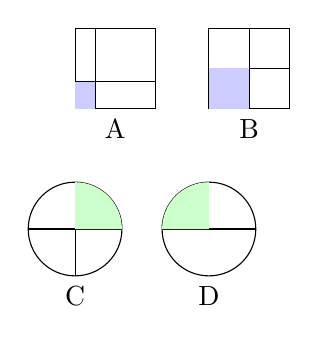
\begin{tikzpicture}[scale=0.85]
% A: Unequal
\draw (0,0) rectangle (1.2,1.2);
\draw (0,0.4) -- (1.2,0.4);
\draw (0.3,0) -- (0.3,1.2);
\fill[blue!20] (0,0) rectangle (0.3,0.4);
\node at (0.6,-0.3) {A};
% B: Equal
\draw (2,0) rectangle (3.2,1.2);
\draw (2,0.6) -- (3.2,0.6);
\draw (2.6,0) -- (2.6,1.2);
\fill[blue!20] (2,0) rectangle (2.6,0.6);
\node at (2.6,-0.3) {B};
% C: Equal
\draw (0,-1.8) circle (0.7);
\draw (0,-1.8) -- (0.7,-1.8);
\draw (0,-1.8) -- (-0.7,-1.8);
\draw (0,-1.8) -- (0,-1.1);
\draw (0,-1.8) -- (0,-2.5);
\fill[green!20] (0,-1.8) -- (0.7,-1.8) arc (0:90:0.7) -- cycle;
\node at (0,-2.8) {C};
% D: Unequal
\draw (2,-1.8) circle (0.7);
\draw (2,-1.8) -- (2.7,-1.8);
\draw (2,-1.8) -- (2,-1.1);
\draw (2,-1.8) -- (1.3,-1.8);
\fill[green!20] (2,-1.8) -- (2,-1.1) arc (90:180:0.7) -- cycle;
\node at (2,-2.8) {D};
\end{tikzpicture}
\end{center}

\column{0.55\textwidth}
\textbf{Questions}
\begin{enumerate}
    \item Which shapes (A, B, C, D) are divided into equal parts? \ashow{B and C}
    \item In shape B, what fraction is shaded? \ashow{$\frac{1}{4}$}
    \item Draw a rectangle divided into 5 equal parts. Shade $\frac{3}{5}$. \ashow{Shade any 3 of the 5 equal parts.}
    \item Which is larger: $\frac{2}{5}$ or $\frac{3}{5}$? \ashow{$\frac{3}{5}$}
    \item Which is larger: $\frac{3}{5}$ or $\frac{3}{4}$? \ashow{$\frac{3}{4}$}
    \item Order the following fractions from smallest to largest: \newline $\frac{1}{100}, \frac{100}{1}, \frac{1}{10}, \frac{10}{1}, \frac{1}{1}$ \ashow{$\frac{1}{100},\ \frac{1}{10},\ \frac{1}{1},\ \frac{10}{1},\ \frac{100}{1}$}
\end{enumerate}
\end{columns}

\end{frame}

%------------------------------------------------

\begin{frame}{Starter 2}
\hypertarget{q-st2}{}

\begin{columns}
\column{0.45\textwidth}
\begin{center}
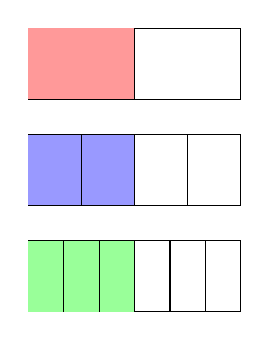
\begin{tikzpicture}[scale=0.9]
% Bar 1/2
\draw (0,0) rectangle (3,1);
\fill[red!40] (0,0) rectangle (1.5,1);

\draw (1.5,0) -- (1.5,1);
% Bar 2/4
\draw (0,-1.5) rectangle (3,-0.5);
\fill[blue!40] (0,-1.5) rectangle (1.5,-0.5);
\draw (0.75,-1.5) -- (0.75,-0.5);
\draw (1.5,-1.5) -- (1.5,-0.5);
\draw (2.25,-1.5) -- (2.25,-0.5);
% Bar 3/6
\draw (0,-3) rectangle (3,-2);
\fill[green!40] (0,-3) rectangle (1.5,-2);
\foreach \x in {0.5,1,1.5,2,2.5} {
    \draw (\x,-3) -- (\x,-2);
}

\end{tikzpicture}
\end{center}

\column{0.55\textwidth}
\textbf{Questions}
\begin{enumerate}
    \item Write the fraction shaded for each bar. \ashow{$\frac{1}{2},\ \frac{2}{4},\ \frac{3}{6}$}
    \item Is the same proportion of each bar shaded? \ashow{Yes}
    \item Use the bars to fill in the blanks: $\frac{\ashowq{1}}{2} = \frac{\ashowq{2}}{4} = \frac{\ashowq{3}}{6}$
    \item Shade $\frac{2}{3}$ of a bar divided into 9 parts. \ashow{Shade 6 parts.}
    \item Find the missing numerator: $\frac{2}{3} = \frac{\ashowq{6}}{9}$
    \item Find the missing numerator: $\frac{1}{3} = \frac{\ashowq{2}}{6}$.
    \item Which two fractions are equivalent: $\frac{1}{2}, \frac{2}{5}, \frac{4}{8}, \frac{3}{6}$? \ashow{$\frac{1}{2} = \frac{4}{8} = \frac{3}{6}$}
\end{enumerate}
\end{columns}

\end{frame}

%------------------------------------------------

\begin{frame}{Starter 3: Comparing Fractions}
\hypertarget{q-st3}{}

\begin{columns}
\column{0.45\textwidth}
\begin{center}
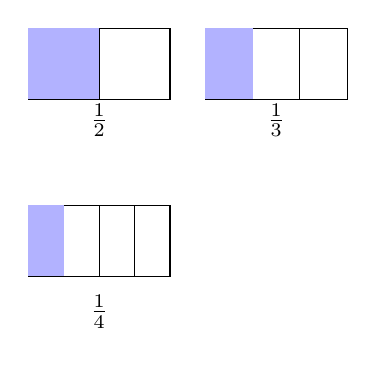
\begin{tikzpicture}[scale=0.9]
\draw (0,0) rectangle (2,1);
\draw (1,0) -- (1,1);
\fill[blue!30] (0,0) rectangle (1,1);
\node at (1,-0.3) {$\frac{1}{2}$};
\draw (2.5,0) rectangle (4.5,1);
\draw (3.17,0) -- (3.17,1);
\draw (3.83,0) -- (3.83,1);
\fill[blue!30] (2.5,0) rectangle (3.17,1);
\node at (3.5,-0.3) {$\frac{1}{3}$};
\draw (0,-2.5) rectangle (2,-1.5);
\draw (0.5,-2.5) -- (0.5,-1.5);
\draw (1,-2.5) -- (1,-1.5);
\draw (1.5,-2.5) -- (1.5,-1.5);
\fill[blue!30] (0,-2.5) rectangle (0.5,-1.5);
\node at (1,-3) {$\frac{1}{4}$};
\end{tikzpicture}
\end{center}

\column{0.55\textwidth}
\textbf{Questions}
\begin{enumerate}
    \item Which is larger: $\frac{1}{2}$ or $\frac{1}{3}$? \ashow{$\frac{1}{2}$}
    \item Compare $\frac{2}{5}$ and $\frac{4}{5}$. Which is bigger? \ashow{$\frac{4}{5}$}
    \item Convert $\frac{3}{4}$ and $\frac{5}{8}$ to a common denominator. Which is larger? \ashow{$\frac{3}{4}=\frac{6}{8}$; larger: $\frac{3}{4}$}
    \item Order from smallest to largest: $\frac{1}{3}, \frac{1}{6}, \frac{1}{2}$. \ashow{$\frac{1}{6},\ \frac{1}{3},\ \frac{1}{2}$}
    \item Sam ate $\frac{2}{3}$ of a pizza, Lee ate $\frac{5}{6}$ of the same pizza. Who ate more? \ashow{Lee ate more.}
    \item Compare $\frac{4}{6}$ and $\frac{2}{3}$. \ashow{Equal: $\frac{4}{6}=\frac{2}{3}$}
\end{enumerate}
\end{columns}

\end{frame}

%------------------------------------------------

\begin{frame}{Starter 4}
\hypertarget{q-st4}{}

\begin{columns}
\column{0.45\textwidth}
\begin{center}
\textbf{Fractions everywhere}
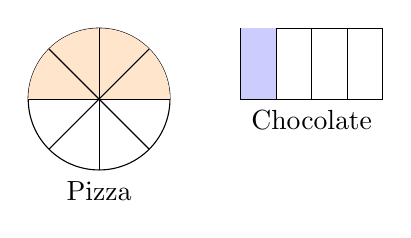
\begin{tikzpicture}[scale=0.9]
\draw (0,0) circle (1);
\fill[orange!20] (0,0) -- (0:1) arc (0:90:1) -- cycle;
\fill[orange!20] (0,0) -- (90:1) arc (90:180:1) -- cycle;
\foreach \a in {0,45,90,135,180,225,270,315} {
    \draw (0,0) -- (\a:1);
}

\node at (0,-1.3) {Pizza};
\draw (2,0) rectangle (4,1);
\draw (2.5,0) -- (2.5,1);
\draw (3,0) -- (3,1);
\draw (3.5,0) -- (3.5,1);
\fill[blue!20] (2,0) rectangle (2.5,1);
\node at (3,-0.3) {Chocolate};
\end{tikzpicture}
\end{center}

\column{0.55\textwidth}
\textbf{Questions}
\begin{enumerate}
    \item A cake is cut into 10 equal slices. If 3 are eaten, what fraction remains? \ablank{$\frac{7}{10}$}.
    \item There are 30 students. $\frac{2}{5}$ walk to school. How many walk? \ashow{12 students walk}
    \item A ruler is 24 cm long. Mark $\frac{1}{2}$ and $\frac{1}{3}$ on it. How many cm is each? \ashow{12 cm and 8 cm}
    \item Which is longer: $\frac{3}{4}$ of an hour or $\frac{2}{3}$ of an hour? (1 hour = 60 mins) \ashow{$\frac{3}{4}$ hour (45 mins) is longer}
    \item You have \$30. You spend $\frac{2}{5}$ on a book. How much do you spend? How much left? \ashow{Spend \$12, left \$18}
    \item A recipe needs $\frac{3}{4}$ cup of milk. You only have a $\frac{1}{4}$ cup measure. How many times must you fill it? \ashow{3 times}
\end{enumerate}
\end{columns}

\end{frame}

%------------------------------------------------

\begin{frame}{Starter 5}
\hypertarget{q-st5}{}

\vspace{-3em}

\begin{columns}

\column{0.25\textwidth}

\begin{center}
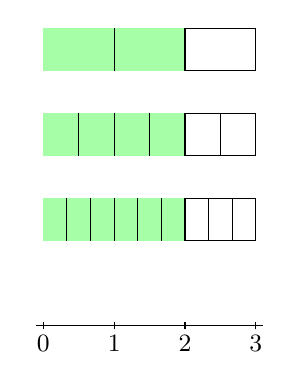
\begin{tikzpicture}[scale=0.9]
% --- Bars for 2/3, 4/6, 6/9 ---
% 2/3 bar
\draw (0,0) rectangle (3,0.6);
\fill[green!35] (0,0) rectangle (2,0.6);

\draw (1,0) -- (1,0.6);
\draw (2,0) -- (2,0.6);

% 4/6 bar
\draw (0,-1.2) rectangle (3,-0.6);
\fill[green!35] (0,-1.2) rectangle (2,-0.6);

\foreach \x in {0.5,1,1.5,2,2.5} \draw (\x,-1.2) -- (\x,-0.6);

% 6/9 bar
\draw (0,-2.4) rectangle (3,-1.8);
\fill[green!35] (0,-2.4) rectangle (2,-1.8);

\foreach \x in {0.333,0.666,1,1.333,1.666,2,2.333,2.666} \draw (\x,-2.4) -- (\x,-1.8);

% --- Compact number line 0 to 3 ---
\draw (-0.1,-3.6) -- (3.1,-3.6);
\foreach \x/\lab in {0/0,1/1,2/2,3/3} {
  \draw (\x,-3.65) -- (\x,-3.55);
  \node at (\x,-3.85) {\small \lab};
}
\end{tikzpicture}
\end{center}

\column{0.75\textwidth}

\small 

\begin{multicols}{2}
\begin{enumerate}
  \item $\dfrac{1}{2}=\dfrac{\ashowq{3}}{6}$
  \item Write the fraction represented by each bar. (Extension) show that they are equivalent \ashow{$\frac{2}{3},\ \frac{4}{6},\ \frac{6}{9}$}
  \item $\dfrac{5}{6}=\dfrac{10}{\ashowq{12}}$


    \item Mark $1\dfrac{2}{3}$ and $2\dfrac{1}{2}$ on the number line. Convert each to an improper fraction. \ashow{$1\frac{2}{3}=\frac{5}{3}$; $2\frac{1}{2}=\frac{5}{2}$}

  \item $\dfrac{2}{3}=\dfrac{\ashowq{8}}{12}$

    \columnbreak

  \item Which are equivalent to $\dfrac{3}{7}$: $\dfrac{9}{21}, \dfrac{6}{14}, \dfrac{12}{28}, \dfrac{8}{21}$? \ashow{$\frac{9}{21},\ \frac{6}{14},\ \frac{12}{28}$}
  \item Write 3 fractions equivalent to $\dfrac{4}{9}$ \ashow{$\frac{8}{18},\ \frac{12}{27},\ \frac{16}{36}$}
  \item Compare ( $<$ $>$ $=$) these fractions: $\dfrac{2}{5}\ \square\ \dfrac{6}{15}$ \ashow{$=$}

  \item Fully simplify $\dfrac{48}{18}$ \ashow{$\frac{8}{3}$ (or $2\frac{2}{3}$)}
\end{enumerate}
\end{multicols}

\end{columns}

\end{frame}

%------------------------------------------------

\begin{frame}{Starter 6}
\hypertarget{q-st6}{}

\vspace{-2.5em}

\begin{columns}

\column{0.25\textwidth}

\begin{center}
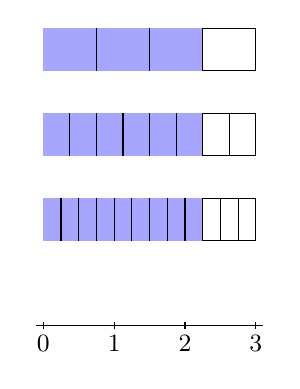
\begin{tikzpicture}[scale=0.9]

% --- Bars for 3/4, 6/8, 9/12 ---
% 3/4
\draw (0,0) rectangle (3,0.6);
\fill[blue!35] (0,0) rectangle (2.25,0.6);
\foreach \x in {0.75,1.5,2.25} \draw (\x,0) -- (\x,0.6);

% 6/8
\draw (0,-1.2) rectangle (3,-0.6);
\fill[blue!35] (0,-1.2) rectangle (2.25,-0.6);
\foreach \x in {0.375,0.75,1.125,1.5,1.875,2.25,2.625} \draw (\x,-1.2) -- (\x,-0.6);

% 9/12
\draw (0,-2.4) rectangle (3,-1.8);
\fill[blue!35] (0,-2.4) rectangle (2.25,-1.8);
\foreach \x in {0.25,0.5,0.75,1,...,2.75} \draw (\x,-2.4) -- (\x,-1.8);

% --- Number Line 0 to 3 ---
\draw (-0.1,-3.6) -- (3.1,-3.6);
\foreach \x/\lab in {0/0,1/1,2/2,3/3} {
  \draw (\x,-3.65) -- (\x,-3.55);
  \node at (\x,-3.85) {\small \lab};
}

\end{tikzpicture}
\end{center}

\column{0.75\textwidth}

\small

\begin{multicols}{2}

\begin{enumerate}

  \item $\dfrac{3}{5}=\dfrac{\ashowq{12}}{20}$

  \item Write the fraction shown by each bar. (Extension) Explain why they represent the same amount. \ashow{$\frac{3}{4},\ \frac{6}{8},\ \frac{9}{12}$}

  \item $\dfrac{4}{7}=\dfrac{\ashowq{12}}{21}$

  \item Mark $1\dfrac{3}{4}$ and $2\dfrac{2}{3}$ on the number line. Convert both to improper fractions. \ashow{$1\frac{3}{4}=\frac{7}{4}$; $2\frac{2}{3}=\frac{8}{3}$}

  \item Fully simplify: $\dfrac{42}{56}$ \ashow{$\frac{3}{4}$}

  \columnbreak

  \item Which are equivalent to $\dfrac{5}{9}$:  
    $\dfrac{10}{18},\ \dfrac{15}{27},\ \dfrac{12}{20},\ \dfrac{25}{45}$? \ashow{$\frac{10}{18},\ \frac{15}{27},\ \frac{25}{45}$}

  \item Write 3 fractions equivalent to $\dfrac{7}{12}$. \ashow{$\frac{14}{24},\ \frac{21}{36},\ \frac{28}{48}$}

  \item Order these fractions in ascending order:  
  \[
  \frac{2}{8},\quad \frac{4}{6},\quad \frac{5}{12}
  \]
  \ashow{$\frac{2}{8},\ \frac{5}{12},\ \frac{4}{6}$}

  \item Compare using $<$, $>$, or $=$:  
  \[
  \frac{9}{14}\ \square\ \frac{19}{28}
  \]
  \ashow{$<$}

\end{enumerate}

\end{multicols}

\end{columns}

\end{frame}

%------------------------------------------------

\begin{frame}{Starter 7}
\hypertarget{q-st7}{}

\vspace{-2.5em}

\begin{columns}

\column{0.25\textwidth}

\begin{center}
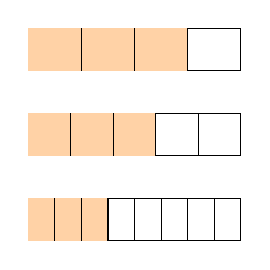
\begin{tikzpicture}[scale=0.9]

% 3/4
\draw (0,0) rectangle (3,0.6);
\fill[orange!35] (0,0) rectangle (2.25,0.6);
\foreach \x in {0.75,1.5,2.25} \draw (\x,0) -- (\x,0.6);

% 3/5
\draw (0,-1.2) rectangle (3,-0.6);
\fill[orange!35] (0,-1.2) rectangle (1.8,-0.6);
\foreach \x in {0.6,1.2,1.8,2.4} \draw (\x,-1.2) -- (\x,-0.6);

% 3/8
\draw (0,-2.4) rectangle (3,-1.8);
\fill[orange!35] (0,-2.4) rectangle (1.125,-1.8);
\foreach \x in {0.375,0.75,1.125,1.5,1.875,2.25,2.625} \draw (\x,-2.4) -- (\x,-1.8);

\end{tikzpicture}
\end{center}

\column{0.75\textwidth}

\small
\begin{multicols}{2}

\begin{enumerate}

\item Write the fraction represented by each bar. \ashow{$\frac{3}{4},\ \frac{3}{5},\ \frac{3}{8}$}

\item Which is largest:  
\[
\frac{3}{4},\quad \frac{3}{5},\quad \frac{3}{8}
\]
\ashow{$\frac{3}{4}$}

\item (Extension) explain why fractions with the same numerator change size when the denominator changes. \ashow{The larger the denominator, the smaller each equal part is.}

\item Compare using $<$, $>$ or $=$:

\[
\frac{5}{6}\ \square\ \frac{5}{9}
\]
\ashow{$>$}

\item Fully simplify: $\frac{18}{24}$ \ashow{$\frac{3}{4}$}

\columnbreak

\item Fully simplify: $
\frac{27}{36}
$ \ashow{$\frac{3}{4}$}

\item Write these as mixed numbers:

\[
\frac{11}{4},\quad \frac{9}{2}
\]
\ashow{$2\frac{3}{4},\ 4\frac{1}{2}$}

\item Convert to improper fractions:

\[
2\frac{3}{5},\quad 1\frac{7}{8}
\]
\ashow{$\frac{13}{5},\ \frac{15}{8}$}

\item Which is bigger:

\[
\frac{7}{10}\ \square\ \frac{7}{12}
\]
\ashow{$\frac{7}{10}$}

\end{enumerate}

\end{multicols}

\end{columns}

\end{frame}

%------------------------------------------------

\begin{frame}{Starter 8}
\hypertarget{q-st8}{}

\vspace{-2.5em}

\begin{columns}

\column{0.25\textwidth}

\begin{center}
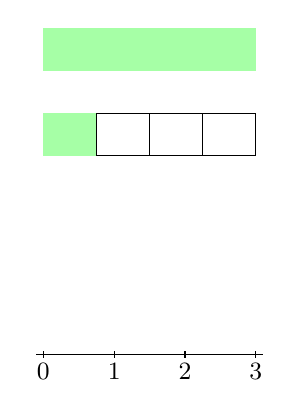
\begin{tikzpicture}[scale=0.9]

% Improper fraction visual (7/4)
\foreach \y in {0,-1.2} {
\draw (0,\y) rectangle (3,\y+0.6);
\foreach \x in {0.75,1.5,2.25} \draw (\x,\y) -- (\x,\y+0.6);
}

\fill[green!35] (0,0) rectangle (3,0.6);
\fill[green!35] (0,-1.2) rectangle (0.75,-0.6);

% number line
\draw (-0.1,-4.0) -- (3.1,-4.0);

\foreach \x/\lab in {0/0,1/1,2/2,3/3} {
\draw (\x,-4.05) -- (\x,-3.95);
\node at (\x,-4.25) {\small \lab};
}

\end{tikzpicture}
\end{center}

\column{0.75\textwidth}

\small
\begin{multicols}{2}

\begin{enumerate}

\item Write the improper fraction shown by the diagram. \ashow{$\frac{5}{4}$}

\item Write the mixed number represented by the green bars in the diagram. \ashow{$1\frac{1}{4}$}

\item Mark $1\frac{1}{4}$ and $2\frac{3}{4}$ on the number line. \ashow{At $1\frac{1}{4}$ and $2\frac{3}{4}$}

\item Convert: $\frac{13}{5}$ to a mixed number. \ashow{$2\frac{3}{5}$}


\item Convert:
\[
3\frac{2}{3}
\]
to an improper fraction. \ashow{$\frac{11}{3}$}

\columnbreak

\item Fully simplify:

\[
\frac{16}{40}
\]
\ashow{$\frac{2}{5}$}

\item Which is greater:

\[
\frac{4}{9}\ \square\ \frac{4}{11}
\]
\ashow{$\frac{4}{9}$}

\item Order from smallest to largest:

\[
\frac{6}{5},\quad 1\frac{1}{2},\quad \frac{7}{4}
\]
\ashow{$\frac{6}{5},\ 1\frac{1}{2},\ \frac{7}{4}$}

\end{enumerate}

\end{multicols}

\end{columns}

\end{frame}

%------------------------------------------------

\begin{frame}{Starter 9}
\hypertarget{q-st9}{}

\vspace{-2.5em}

\begin{columns}

\column{0.25\textwidth}

\begin{center}
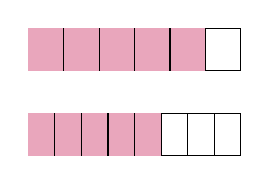
\begin{tikzpicture}[scale=0.9]

% 5/6 bar
\draw (0,0) rectangle (3,0.6);
\fill[purple!35] (0,0) rectangle (2.5,0.6);

\foreach \x in {0.5,1,1.5,2,2.5} \draw (\x,0) -- (\x,0.6);

% 5/8 bar
\draw (0,-1.2) rectangle (3,-0.6);
\fill[purple!35] (0,-1.2) rectangle (1.875,-0.6);

\foreach \x in {0.375,0.75,1.125,1.5,1.875,2.25,2.625} \draw (\x,-1.2) -- (\x,-0.6);

\end{tikzpicture}
\end{center}

\column{0.75\textwidth}

\small
\begin{multicols}{2}

\begin{enumerate}

\item Write the fractions shown by the bars. \ashow{$\frac{5}{6}$ and $\frac{5}{8}$}

\item Which is larger:

\[
\frac{5}{6}\ \square\ \frac{5}{8}
\]
\ashow{$>$}

\item Write 3 fractions equivalent to:

\[
\frac{2}{5}
\]
\ashow{$\frac{4}{10},\ \frac{6}{15},\ \frac{8}{20}$}

\item Fully simplify:
\[
\frac{54}{72}
\]
\ashow{$\frac{3}{4}$}

\item Convert to mixed numbers:

\[
\frac{17}{6},\quad \frac{22}{9}
\]
\ashow{$2\frac{5}{6},\ 2\frac{4}{9}$}

\item Convert to improper fractions:

\[
4\frac{1}{3},\quad 2\frac{5}{6}
\]
\ashow{$\frac{13}{3},\ \frac{17}{6}$}

\item Order from smallest to largest:

\[
\frac{123}{1234},\quad \frac{321}{1234},\quad \frac{111}{1234}
\]
\ashow{$\frac{111}{1234},\ \frac{123}{1234},\ \frac{321}{1234}$}

\item Challenge:

Which is larger?

\[
2\frac{1}{4}\ \square\ 2\frac{2}{5}
\]
\ashow{$2\frac{2}{5}$}

\end{enumerate}

\end{multicols}

\end{columns}

\end{frame}

% ================================================================
% Worked solutions
% ================================================================

\begin{frame}{Worked Solution: Starter 1, Question 1}
\hypertarget{work-st1}{}

\textbf{Question:} Which shapes (A, B, C, D) are divided into equal parts?

\textbf{Worked Solution:}
\begin{itemize}
  \item A is not divided into equal parts.
  \item B is divided into 4 congruent squares, so it is equal.
  \item C is divided into 4 equal quarter-circles, so it is equal.
  \item D is divided into unequal sectors.
\end{itemize}
So the shapes divided into equal parts are \textbf{B and C}.
\end{frame}

\begin{frame}{Worked Solution: Starter 1, Question 2}

\textbf{Question:} In shape B, what fraction is shaded?

\textbf{Worked Solution:}
Shape B is a square divided into 4 equal smaller squares. One of the 4 smaller squares is shaded, so the shaded fraction is  
\[
\frac{1}{4}.
\]
\end{frame}

\begin{frame}{Worked Solution: Starter 1, Question 3}

\textbf{Question:} Draw a rectangle divided into 5 equal parts. Shade $\frac{3}{5}$.

\textbf{Worked Solution:}
Draw a rectangle and divide it into 5 equal vertical strips. Shade any 3 of those 5 strips.  
Since each strip is $\frac{1}{5}$, three strips represent  
\[
\frac{1}{5} + \frac{1}{5} + \frac{1}{5} = \frac{3}{5}.
\]
\end{frame}

\begin{frame}{Worked Solution: Starter 1, Question 4}

\textbf{Question:} Which is larger: $\frac{2}{5}$ or $\frac{3}{5}$?

\textbf{Worked Solution:}
Both fractions have the same denominator, $5$.  
Compare the numerators: $2 < 3$.  
Therefore  
\[
\frac{2}{5} < \frac{3}{5}.
\]
So $\frac{3}{5}$ is larger.
\end{frame}

\begin{frame}{Worked Solution: Starter 1, Question 5}

\textbf{Question:} Which is larger: $\frac{3}{5}$ or $\frac{3}{4}$?

\textbf{Worked Solution:}
Both fractions have the same numerator, $3$.  
The denominator $4$ is smaller than $5$, so $\frac{3}{4}$ has larger equal parts than $\frac{3}{5}$.  
Thus  
\[
\frac{3}{4} > \frac{3}{5}.
\]
\end{frame}

\begin{frame}{Worked Solution: Starter 1, Question 6}

\textbf{Question:} Order $\frac{1}{100}, \frac{100}{1}, \frac{1}{10}, \frac{10}{1}, \frac{1}{1}$ from smallest to largest.

\textbf{Worked Solution:}
Write each as a decimal or whole number:
\[
\frac{1}{100}=0.01,\quad \frac{1}{10}=0.1,\quad \frac{1}{1}=1,\quad \frac{10}{1}=10,\quad \frac{100}{1}=100.
\]
So the ascending order is
\[
\frac{1}{100},\ \frac{1}{10},\ \frac{1}{1},\ \frac{10}{1},\ \frac{100}{1}.
\]
\end{frame}

%------------------------------------------------

\begin{frame}{Worked Solution: Starter 2, Question 1}
\hypertarget{work-st2}{}

\textbf{Question:} Write the fraction shaded for each bar.

\textbf{Worked Solution:}
\begin{itemize}
  \item Bar 1: 1 part shaded out of 2 equal parts, so $\frac{1}{2}$.
  \item Bar 2: 2 parts shaded out of 4 equal parts, so $\frac{2}{4}$.
  \item Bar 3: 3 parts shaded out of 6 equal parts, so $\frac{3}{6}$.
\end{itemize}
\end{frame}

\begin{frame}{Worked Solution: Starter 2, Question 2}

\textbf{Question:} Is the same proportion of each bar shaded?

\textbf{Worked Solution:}
Yes. Each shaded part is half of its bar:
\[
\frac{1}{2} = \frac{2}{4} = \frac{3}{6}.
\]
The fractions are equivalent.
\end{frame}

\begin{frame}{Worked Solution: Starter 2, Question 3}

\textbf{Question:} Fill the blanks: $\frac{?}{2} = \frac{?}{4} = \frac{?}{6}$.

\textbf{Worked Solution:}
The bars show
\[
\frac{1}{2} = \frac{2}{4} = \frac{3}{6}.
\]
So the missing numbers are $1$, $2$, and $3$.
\end{frame}

\begin{frame}{Worked Solution: Starter 2, Question 4}

\textbf{Question:} Shade $\frac{2}{3}$ of a bar divided into 9 parts.

\textbf{Worked Solution:}
\[
\frac{2}{3} \text{ of } 9 = \frac{2}{3} \times 9 = 6.
\]
Shade 6 of the 9 equal parts.
\end{frame}

\begin{frame}{Worked Solution: Starter 2, Question 5}

\textbf{Question:} Find the missing numerator: $\frac{2}{3} = \frac{?}{9}$.

\textbf{Worked Solution:}
To change $3$ into $9$, multiply by $3$.  
Multiply the numerator by $3$ too:
\[
\frac{2}{3} = \frac{2 \times 3}{3 \times 3} = \frac{6}{9}.
\]
So the missing numerator is $6$.
\end{frame}

\begin{frame}{Worked Solution: Starter 2, Question 6}

\textbf{Question:} Find the missing numerator: $\frac{1}{3} = \frac{?}{6}$.

\textbf{Worked Solution:}
To change $3$ into $6$, multiply by $2$.  
Multiply the numerator by $2$ too:
\[
\frac{1}{3} = \frac{1 \times 2}{3 \times 2} = \frac{2}{6}.
\]
So the missing numerator is $2$.
\end{frame}

\begin{frame}{Worked Solution: Starter 2, Question 7}

\textbf{Question:} Which fractions are equivalent: $\frac{1}{2}, \frac{2}{5}, \frac{4}{8}, \frac{3}{6}$?

\textbf{Worked Solution:}
\[
\frac{4}{8} = \frac{1}{2} \quad \text{and} \quad \frac{3}{6} = \frac{1}{2}.
\]
So the equivalent fractions are
\[
\frac{1}{2},\ \frac{4}{8},\ \frac{3}{6}.
\]
The fraction $\frac{2}{5}$ is not equivalent.
\end{frame}

%------------------------------------------------

\begin{frame}{Worked Solution: Starter 3, Question 1}
\hypertarget{work-st3}{}

\textbf{Question:} Which is larger: $\frac{1}{2}$ or $\frac{1}{3}$?

\textbf{Worked Solution:}
Same numerator, so compare denominators.  
Since $2 < 3$, the fraction with denominator $2$ is larger:
\[
\frac{1}{2} > \frac{1}{3}.
\]
So $\frac{1}{2}$ is larger.
\end{frame}

\begin{frame}{Worked Solution: Starter 3, Question 2}

\textbf{Question:} Compare $\frac{2}{5}$ and $\frac{4}{5}$.

\textbf{Worked Solution:}
Same denominator $5$. Compare numerators: $2 < 4$.  
Therefore
\[
\frac{2}{5} < \frac{4}{5}.
\]
So $\frac{4}{5}$ is bigger.
\end{frame}

\begin{frame}{Worked Solution: Starter 3, Question 3}

\textbf{Question:} Convert $\frac{3}{4}$ and $\frac{5}{8}$ to a common denominator. Which is larger?

\textbf{Worked Solution:}
A common denominator is $8$:
\[
\frac{3}{4} = \frac{3 \times 2}{4 \times 2} = \frac{6}{8}.
\]
Now compare:
\[
\frac{6}{8} > \frac{5}{8}.
\]
So $\frac{3}{4}$ is larger.
\end{frame}

\begin{frame}{Worked Solution: Starter 3, Question 4}

\textbf{Question:} Order $\frac{1}{3}, \frac{1}{6}, \frac{1}{2}$ from smallest to largest.

\textbf{Worked Solution:}
All have numerator $1$. The larger the denominator, the smaller the fraction.  
\[
\frac{1}{6} < \frac{1}{3} < \frac{1}{2}.
\]
So the order is
\[
\frac{1}{6},\ \frac{1}{3},\ \frac{1}{2}.
\]
\end{frame}

\begin{frame}{Worked Solution: Starter 3, Question 5}

\textbf{Question:} Sam ate $\frac{2}{3}$ of a pizza, Lee ate $\frac{5}{6}$ of the same pizza. Who ate more?

\textbf{Worked Solution:}
Write $\frac{2}{3}$ with denominator $6$:
\[
\frac{2}{3} = \frac{4}{6}.
\]
Lee ate $\frac{5}{6} > \frac{4}{6}$, so Lee ate more.
\end{frame}

\begin{frame}{Worked Solution: Starter 3, Question 6}

\textbf{Question:} Compare $\frac{4}{6}$ and $\frac{2}{3}$.

\textbf{Worked Solution:}
Simplify $\frac{4}{6}$ by dividing numerator and denominator by $2$:
\[
\frac{4}{6} = \frac{2}{3}.
\]
So they are equal.
\end{frame}

%------------------------------------------------

\begin{frame}{Worked Solution: Starter 4, Question 1}
\hypertarget{work-st4}{}

\textbf{Question:} A cake is cut into 10 equal slices. If 3 are eaten, what fraction remains?

\textbf{Worked Solution:}
Slices remaining:
\[
10 - 3 = 7.
\]
So the fraction remaining is
\[
\frac{7}{10}.
\]
\end{frame}

\begin{frame}{Worked Solution: Starter 4, Question 2}

\textbf{Question:} There are 30 students. $\frac{2}{5}$ walk to school. How many walk?

\textbf{Worked Solution:}
\[
\frac{2}{5} \text{ of } 30 = \frac{2}{5} \times 30 = 2 \times 6 = 12.
\]
So 12 students walk to school.
\end{frame}

\begin{frame}{Worked Solution: Starter 4, Question 3}

\textbf{Question:} A ruler is 24 cm long. Mark $\frac{1}{2}$ and $\frac{1}{3}$ on it. How many cm is each?

\textbf{Worked Solution:}
\[
\frac{1}{2} \text{ of } 24 = 12 \text{ cm}.
\]
\[
\frac{1}{3} \text{ of } 24 = 8 \text{ cm}.
\]
Mark at 12 cm and 8 cm.
\end{frame}

\begin{frame}{Worked Solution: Starter 4, Question 4}

\textbf{Question:} Which is longer: $\frac{3}{4}$ of an hour or $\frac{2}{3}$ of an hour?

\textbf{Worked Solution:}
\[
\frac{3}{4} \text{ hour} = \frac{3}{4} \times 60 = 45 \text{ minutes}.
\]
\[
\frac{2}{3} \text{ hour} = \frac{2}{3} \times 60 = 40 \text{ minutes}.
\]
So $\frac{3}{4}$ of an hour is longer.
\end{frame}

\begin{frame}{Worked Solution: Starter 4, Question 5}

\textbf{Question:} You have \$30. You spend $\frac{2}{5}$ on a book. How much do you spend? How much left?

\textbf{Worked Solution:}
\[
\text{Spent} = \frac{2}{5} \times 30 = 12.
\]
\[
\text{Left} = 30 - 12 = 18.
\]
So you spend \$12 and have \$18 left.
\end{frame}

\begin{frame}{Worked Solution: Starter 4, Question 6}

\textbf{Question:} A recipe needs $\frac{3}{4}$ cup of milk. You have a $\frac{1}{4}$ cup measure. How many times must you fill it?

\textbf{Worked Solution:}
\[
\frac{3}{4} \div \frac{1}{4} = \frac{3}{4} \times \frac{4}{1} = 3.
\]
Fill the $\frac{1}{4}$ cup measure 3 times.
\end{frame}

%------------------------------------------------

\begin{frame}{Worked Solution: Starter 5, Question 1}
\hypertarget{work-st5}{}

\textbf{Question:} $\frac{1}{2} = \frac{?}{6}$.

\textbf{Worked Solution:}
Multiply numerator and denominator by $3$:
\[
\frac{1}{2} = \frac{1 \times 3}{2 \times 3} = \frac{3}{6}.
\]
So the missing number is $3$.
\end{frame}

\begin{frame}{Worked Solution: Starter 5, Question 2}

\textbf{Question:} Write the fraction represented by each bar and show they are equivalent.

\textbf{Worked Solution:}
\[
\frac{2}{3},\quad \frac{4}{6},\quad \frac{6}{9}.
\]
Simplify:
\[
\frac{4}{6} = \frac{2}{3}, \qquad \frac{6}{9} = \frac{2}{3}.
\]
So all three bars show the same amount.
\end{frame}

\begin{frame}{Worked Solution: Starter 5, Question 3}

\textbf{Question:} $\frac{5}{6} = \frac{10}{?}$.

\textbf{Worked Solution:}
Multiply numerator and denominator by $2$:
\[
\frac{5}{6} = \frac{5 \times 2}{6 \times 2} = \frac{10}{12}.
\]
So the missing number is $12$.
\end{frame}

\begin{frame}{Worked Solution: Starter 5, Question 4}

\textbf{Question:} Mark $1\frac{2}{3}$ and $2\frac{1}{2}$ on the number line. Convert each to an improper fraction.

\textbf{Worked Solution:}
\[
1\frac{2}{3} = \frac{1 \times 3 + 2}{3} = \frac{5}{3}.
\]
\[
2\frac{1}{2} = \frac{2 \times 2 + 1}{2} = \frac{5}{2}.
\]
Mark $1\frac{2}{3}$ between $1$ and $2$, and mark $2\frac{1}{2}$ halfway between $2$ and $3$.
\end{frame}

\begin{frame}{Worked Solution: Starter 5, Question 5}

\textbf{Question:} $\frac{2}{3} = \frac{?}{12}$.

\textbf{Worked Solution:}
Multiply numerator and denominator by $4$:
\[
\frac{2}{3} = \frac{2 \times 4}{3 \times 4} = \frac{8}{12}.
\]
So the missing number is $8$.
\end{frame}

\begin{frame}{Worked Solution: Starter 5, Question 6}

\textbf{Question:} Which are equivalent to $\frac{3}{7}$: $\frac{9}{21}, \frac{6}{14}, \frac{12}{28}, \frac{8}{21}$?

\textbf{Worked Solution:}
\[
\frac{9}{21} = \frac{3}{7}, \qquad
\frac{6}{14} = \frac{3}{7}, \qquad
\frac{12}{28} = \frac{3}{7}.
\]
But $\frac{8}{21}$ cannot be simplified to $\frac{3}{7}$.  
So the equivalent fractions are $\frac{9}{21}$, $\frac{6}{14}$, and $\frac{12}{28}$.
\end{frame}

\begin{frame}{Worked Solution: Starter 5, Question 7}

\textbf{Question:} Write 3 fractions equivalent to $\frac{4}{9}$.

\textbf{Worked Solution:}
Multiply numerator and denominator by $2$, $3$, and $4$:
\[
\frac{4}{9} = \frac{8}{18} = \frac{12}{27} = \frac{16}{36}.
\]
\end{frame}

\begin{frame}{Worked Solution: Starter 5, Question 8}

\textbf{Question:} Compare $\frac{2}{5}$ and $\frac{6}{15}$.

\textbf{Worked Solution:}
Simplify $\frac{6}{15}$ by dividing by $3$:
\[
\frac{6}{15} = \frac{2}{5}.
\]
So $\frac{2}{5} = \frac{6}{15}$, and the correct symbol is $=$.
\end{frame}

\begin{frame}{Worked Solution: Starter 5, Question 9}

\textbf{Question:} Fully simplify $\frac{48}{18}$.

\textbf{Worked Solution:}
Divide numerator and denominator by $6$:
\[
\frac{48}{18} = \frac{8}{3}.
\]
As a mixed number:
\[
\frac{8}{3} = 2\frac{2}{3}.
\]
\end{frame}

%------------------------------------------------

\begin{frame}{Worked Solution: Starter 6, Question 1}
\hypertarget{work-st6}{}

\textbf{Question:} $\frac{3}{5} = \frac{?}{20}$.

\textbf{Worked Solution:}
Multiply numerator and denominator by $4$:
\[
\frac{3}{5} = \frac{3 \times 4}{5 \times 4} = \frac{12}{20}.
\]
So the missing number is $12$.
\end{frame}

\begin{frame}{Worked Solution: Starter 6, Question 2}

\textbf{Question:} Write the fraction shown by each bar and explain why they represent the same amount.

\textbf{Worked Solution:}
\[
\frac{3}{4},\quad \frac{6}{8},\quad \frac{9}{12}.
\]
\[
\frac{6}{8} = \frac{3}{4}, \qquad \frac{9}{12} = \frac{3}{4}.
\]
They all reduce to $\frac{3}{4}$, so they represent the same shaded amount.
\end{frame}

\begin{frame}{Worked Solution: Starter 6, Question 3}

\textbf{Question:} $\frac{4}{7} = \frac{?}{21}$.

\textbf{Worked Solution:}
Multiply numerator and denominator by $3$:
\[
\frac{4}{7} = \frac{4 \times 3}{7 \times 3} = \frac{12}{21}.
\]
So the missing number is $12$.
\end{frame}

\begin{frame}{Worked Solution: Starter 6, Question 4}

\textbf{Question:} Mark $1\frac{3}{4}$ and $2\frac{2}{3}$ on the number line. Convert both to improper fractions.

\textbf{Worked Solution:}
\[
1\frac{3}{4} = \frac{1 \times 4 + 3}{4} = \frac{7}{4}.
\]
\[
2\frac{2}{3} = \frac{2 \times 3 + 2}{3} = \frac{8}{3}.
\]
Mark $1\frac{3}{4}=1.75$ and $2\frac{2}{3}\approx 2.67$.
\end{frame}

\begin{frame}{Worked Solution: Starter 6, Question 5}

\textbf{Question:} Fully simplify $\frac{42}{56}$.

\textbf{Worked Solution:}
Divide numerator and denominator by $14$:
\[
\frac{42}{56} = \frac{3}{4}.
\]
So $\frac{42}{56}$ simplifies to $\frac{3}{4}$.
\end{frame}

\begin{frame}{Worked Solution: Starter 6, Question 6}

\textbf{Question:} Which are equivalent to $\frac{5}{9}$: $\frac{10}{18}, \frac{15}{27}, \frac{12}{20}, \frac{25}{45}$?

\textbf{Worked Solution:}
\[
\frac{10}{18} = \frac{5}{9}, \qquad
\frac{15}{27} = \frac{5}{9}, \qquad
\frac{25}{45} = \frac{5}{9}.
\]
But
\[
\frac{12}{20} = \frac{3}{5},
\]
which is not equivalent to $\frac{5}{9}$.  
So the equivalent fractions are $\frac{10}{18}$, $\frac{15}{27}$, and $\frac{25}{45}$.
\end{frame}

\begin{frame}{Worked Solution: Starter 6, Question 7}

\textbf{Question:} Write 3 fractions equivalent to $\frac{7}{12}$.

\textbf{Worked Solution:}
\[
\frac{7}{12} = \frac{14}{24} = \frac{21}{36} = \frac{28}{48}.
\]
These are found by multiplying numerator and denominator by $2$, $3$, and $4$.
\end{frame}

\begin{frame}{Worked Solution: Starter 6, Question 8}

\textbf{Question:} Order $\frac{2}{8}, \frac{4}{6}, \frac{5}{12}$ in ascending order.

\textbf{Worked Solution:}
Use denominator $12$:
\[
\frac{2}{8} = \frac{1}{4} = \frac{3}{12}, \qquad
\frac{4}{6} = \frac{8}{12}, \qquad
\frac{5}{12} = \frac{5}{12}.
\]
Therefore,
\[
\frac{3}{12} < \frac{5}{12} < \frac{8}{12}.
\]
So the order is
\[
\frac{2}{8},\ \frac{5}{12},\ \frac{4}{6}.
\]
\end{frame}

\begin{frame}{Worked Solution: Starter 6, Question 9}

\textbf{Question:} Compare $\frac{9}{14}$ and $\frac{19}{28}$.

\textbf{Worked Solution:}
\[
\frac{9}{14} = \frac{18}{28}.
\]
Since
\[
\frac{18}{28} < \frac{19}{28},
\]
we have
\[
\frac{9}{14} < \frac{19}{28}.
\]
So the correct symbol is $<$.
\end{frame}

%------------------------------------------------

\begin{frame}{Worked Solution: Starter 7, Question 1}
\hypertarget{work-st7}{}

\textbf{Question:} Write the fraction represented by each bar.

\textbf{Worked Solution:}
The bars are divided into $4$, $5$, and $8$ equal parts, with $3$ parts shaded:
\[
\frac{3}{4},\quad \frac{3}{5},\quad \frac{3}{8}.
\]
\end{frame}

\begin{frame}{Worked Solution: Starter 7, Question 2}

\textbf{Question:} Which is largest: $\frac{3}{4}, \frac{3}{5}, \frac{3}{8}$?

\textbf{Worked Solution:}
All have numerator $3$. The smaller the denominator, the larger each equal part is.  
Since
\[
4 < 5 < 8,
\]
we have
\[
\frac{3}{4} > \frac{3}{5} > \frac{3}{8}.
\]
So $\frac{3}{4}$ is the largest.
\end{frame}

\begin{frame}{Worked Solution: Starter 7, Question 3}

\textbf{Question:} Explain why fractions with the same numerator change size when the denominator changes.

\textbf{Worked Solution:}
The numerator tells the number of equal parts taken.  
The denominator tells how many equal parts the whole is divided into.  
If the denominator increases, the whole is divided into more parts, so each part is smaller.  
Therefore, with the same numerator, a larger denominator gives a smaller fraction.
\end{frame}

\begin{frame}{Worked Solution: Starter 7, Question 4}

\textbf{Question:} Compare $\frac{5}{6}$ and $\frac{5}{9}$.

\textbf{Worked Solution:}
Same numerator $5$; compare denominators.  
Since $6 < 9$,
\[
\frac{5}{6} > \frac{5}{9}.
\]
So the correct symbol is $>$.
\end{frame}

\begin{frame}{Worked Solution: Starter 7, Question 5}

\textbf{Question:} Fully simplify $\frac{18}{24}$.

\textbf{Worked Solution:}
Divide numerator and denominator by $6$:
\[
\frac{18}{24} = \frac{3}{4}.
\]
\end{frame}

\begin{frame}{Worked Solution: Starter 7, Question 6}

\textbf{Question:} Fully simplify $\frac{27}{36}$.

\textbf{Worked Solution:}
Divide numerator and denominator by $9$:
\[
\frac{27}{36} = \frac{3}{4}.
\]
\end{frame}

\begin{frame}{Worked Solution: Starter 7, Question 7}

\textbf{Question:} Write $\frac{11}{4}$ and $\frac{9}{2}$ as mixed numbers.

\textbf{Worked Solution:}
\[
11 \div 4 = 2 \text{ remainder } 3, \quad \text{so } \frac{11}{4} = 2\frac{3}{4}.
\]
\[
9 \div 2 = 4 \text{ remainder } 1, \quad \text{so } \frac{9}{2} = 4\frac{1}{2}.
\]
\end{frame}

\begin{frame}{Worked Solution: Starter 7, Question 8}

\textbf{Question:} Convert $2\frac{3}{5}$ and $1\frac{7}{8}$ to improper fractions.

\textbf{Worked Solution:}
\[
2\frac{3}{5} = \frac{2 \times 5 + 3}{5} = \frac{13}{5}.
\]
\[
1\frac{7}{8} = \frac{1 \times 8 + 7}{8} = \frac{15}{8}.
\]
\end{frame}

\begin{frame}{Worked Solution: Starter 7, Question 9}

\textbf{Question:} Which is bigger: $\frac{7}{10}$ or $\frac{7}{12}$?

\textbf{Worked Solution:}
Same numerator $7$. Since $10 < 12$,
\[
\frac{7}{10} > \frac{7}{12}.
\]
So $\frac{7}{10}$ is bigger.
\end{frame}

%------------------------------------------------

\begin{frame}{Worked Solution: Starter 8, Question 1}
\hypertarget{work-st8}{}

\textbf{Question:} Write the improper fraction shown by the diagram.

\textbf{Worked Solution:}
The first full bar is shaded:
\[
\frac{4}{4}.
\]
The second bar has 1 of 4 quarters shaded:
\[
\frac{1}{4}.
\]
Total shaded:
\[
\frac{4}{4} + \frac{1}{4} = \frac{5}{4}.
\]
\end{frame}

\begin{frame}{Worked Solution: Starter 8, Question 2}

\textbf{Question:} Write the mixed number represented by the green bars in the diagram.

\textbf{Worked Solution:}
\[
\frac{5}{4} = 1 \text{ whole and } \frac{1}{4} = 1\frac{1}{4}.
\]
\end{frame}

\begin{frame}{Worked Solution: Starter 8, Question 3}

\textbf{Question:} Mark $1\frac{1}{4}$ and $2\frac{3}{4}$ on the number line.

\textbf{Worked Solution:}
\[
1\frac{1}{4} = 1.25, \qquad 2\frac{3}{4} = 2.75.
\]
Mark these points on the number line between $1$ and $2$, and between $2$ and $3$.
\end{frame}

\begin{frame}{Worked Solution: Starter 8, Question 4}

\textbf{Question:} Convert $\frac{13}{5}$ to a mixed number.

\textbf{Worked Solution:}
\[
13 \div 5 = 2 \text{ remainder } 3.
\]
So
\[
\frac{13}{5} = 2\frac{3}{5}.
\]
\end{frame}

\begin{frame}{Worked Solution: Starter 8, Question 5}

\textbf{Question:} Convert $3\frac{2}{3}$ to an improper fraction.

\textbf{Worked Solution:}
\[
3\frac{2}{3} = \frac{3 \times 3 + 2}{3} = \frac{11}{3}.
\]
\end{frame}

\begin{frame}{Worked Solution: Starter 8, Question 6}

\textbf{Question:} Fully simplify $\frac{16}{40}$.

\textbf{Worked Solution:}
Divide numerator and denominator by $8$:
\[
\frac{16}{40} = \frac{2}{5}.
\]
\end{frame}

\begin{frame}{Worked Solution: Starter 8, Question 7}

\textbf{Question:} Which is greater: $\frac{4}{9}$ or $\frac{4}{11}$?

\textbf{Worked Solution:}
Same numerator $4$. Since $9 < 11$,
\[
\frac{4}{9} > \frac{4}{11}.
\]
So $\frac{4}{9}$ is greater.
\end{frame}

\begin{frame}{Worked Solution: Starter 8, Question 8}

\textbf{Question:} Order $\frac{6}{5}$, $1\frac{1}{2}$, and $\frac{7}{4}$ from smallest to largest.

\textbf{Worked Solution:}
Use denominator $20$:
\[
\frac{6}{5} = \frac{24}{20}, \qquad
1\frac{1}{2} = \frac{3}{2} = \frac{30}{20}, \qquad
\frac{7}{4} = \frac{35}{20}.
\]
Therefore,
\[
\frac{24}{20} < \frac{30}{20} < \frac{35}{20}.
\]
So the order is
\[
\frac{6}{5},\ 1\frac{1}{2},\ \frac{7}{4}.
\]
\end{frame}

%------------------------------------------------

\begin{frame}{Worked Solution: Starter 9, Question 1}
\hypertarget{work-st9}{}

\textbf{Question:} Write the fractions shown by the bars.

\textbf{Worked Solution:}
The first bar has 5 parts shaded out of 6 equal parts:
\[
\frac{5}{6}.
\]
The second bar has 5 parts shaded out of 8 equal parts:
\[
\frac{5}{8}.
\]
\end{frame}

\begin{frame}{Worked Solution: Starter 9, Question 2}

\textbf{Question:} Which is larger: $\frac{5}{6}$ or $\frac{5}{8}$?

\textbf{Worked Solution:}
Same numerator $5$. Since $6 < 8$,
\[
\frac{5}{6} > \frac{5}{8}.
\]
So the correct symbol is $>$.
\end{frame}

\begin{frame}{Worked Solution: Starter 9, Question 3}

\textbf{Question:} Write 3 fractions equivalent to $\frac{2}{5}$.

\textbf{Worked Solution:}
\[
\frac{2}{5} = \frac{4}{10} = \frac{6}{15} = \frac{8}{20}.
\]
These are found by multiplying the numerator and denominator by $2$, $3$, and $4$.
\end{frame}

\begin{frame}{Worked Solution: Starter 9, Question 4}

\textbf{Question:} Fully simplify $\frac{54}{72}$.

\textbf{Worked Solution:}
Divide numerator and denominator by $18$:
\[
\frac{54}{72} = \frac{3}{4}.
\]
\end{frame}

\begin{frame}{Worked Solution: Starter 9, Question 5}

\textbf{Question:} Convert $\frac{17}{6}$ and $\frac{22}{9}$ to mixed numbers.

\textbf{Worked Solution:}
\[
17 \div 6 = 2 \text{ remainder } 5, \quad \text{so } \frac{17}{6} = 2\frac{5}{6}.
\]
\[
22 \div 9 = 2 \text{ remainder } 4, \quad \text{so } \frac{22}{9} = 2\frac{4}{9}.
\]
\end{frame}

\begin{frame}{Worked Solution: Starter 9, Question 6}

\textbf{Question:} Convert $4\frac{1}{3}$ and $2\frac{5}{6}$ to improper fractions.

\textbf{Worked Solution:}
\[
4\frac{1}{3} = \frac{4 \times 3 + 1}{3} = \frac{13}{3}.
\]
\[
2\frac{5}{6} = \frac{2 \times 6 + 5}{6} = \frac{17}{6}.
\]
\end{frame}

\begin{frame}{Worked Solution: Starter 9, Question 7}

\textbf{Question:} Order $\frac{123}{1234}, \frac{321}{1234}, \frac{111}{1234}$ from smallest to largest.

\textbf{Worked Solution:}
All fractions have the same denominator, $1234$.  
Compare numerators:
\[
111 < 123 < 321.
\]
So the order is
\[
\frac{111}{1234},\ \frac{123}{1234},\ \frac{321}{1234}.
\]
\end{frame}

\begin{frame}{Worked Solution: Starter 9, Question 8}

\textbf{Question:} Which is larger: $2\frac{1}{4}$ or $2\frac{2}{5}$?

\textbf{Worked Solution:}
Both have whole part $2$. Compare the fractional parts:
\[
\frac{1}{4} = \frac{5}{20}, \qquad \frac{2}{5} = \frac{8}{20}.
\]
Since
\[
\frac{8}{20} > \frac{5}{20},
\]
we have
\[
2\frac{2}{5} > 2\frac{1}{4}.
\]
So $2\frac{2}{5}$ is larger.
\end{frame}

\end{document}